\emph{Konstruktion:} Man zeichnet $\vec F_1$ und hängt $\vec F_2$ an ihre Spitze an. Die Summe $\vec F_1+\vec F_2$ reicht vom Anfangspunkt bis zur Spitze von $\vec F_2$. Die dritte Kraft $\vec F_3$ ist gleich lang, aber entgegengesetzt gerichtet (Massstab: ein Häuschen pro Newton).
\begin{center}
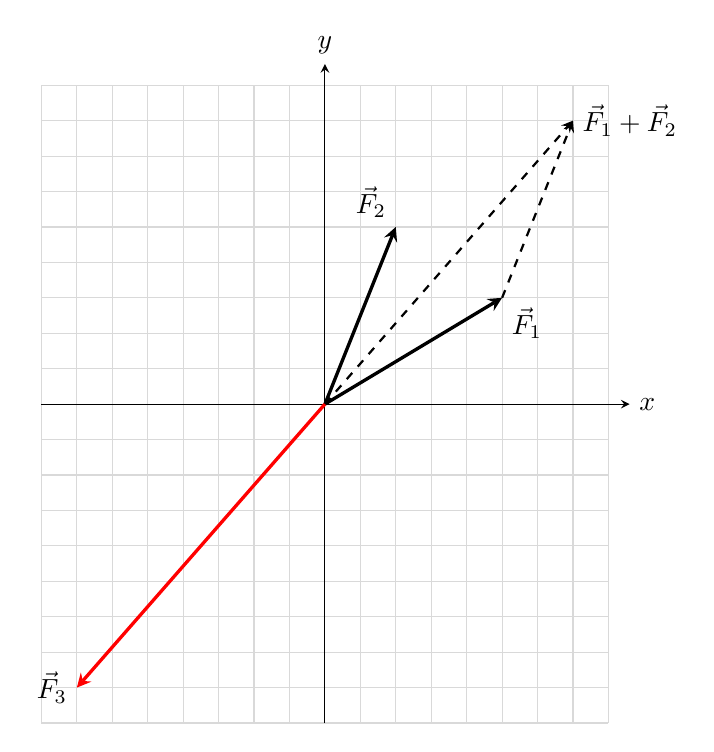
\begin{tikzpicture}[>=stealth, scale=0.45]
 \draw[gray!30] (-8,-9) grid (8,9);
 \draw[->] (-8,0) -- (8.6,0) node[right] {$x$};
 \draw[->] (0,-9) -- (0,9.6) node[above] {$y$};
 \draw[->, very thick] (0,0) -- (5,3);
 \node[below right] at (5,3) {$\vec F_1$};
 \draw[->, very thick] (0,0) -- (2,5);
 \node[above left] at (2,5) {$\vec F_2$};
 \draw[->, thick, dashed] (5,3) -- (7,8);
 \draw[->, thick, dashed] (0,0) -- (7,8);
 \node[right] at (7,8) {$\vec F_1+\vec F_2$};
 \draw[->, very thick, red] (0,0) -- (-7,-8);
 \node[left] at (-7,-8) {$\vec F_3$};
\end{tikzpicture}
\end{center}

\emph{Rechnung:} Im Gleichgewicht ist die Summe aller Kräfte null, $\vec F_1+\vec F_2+\vec F_3 = \vec 0$. Komponentenweise:
\begin{align}
 F_{3x} &= \FcxF = -\left(\Fax+\Fbx\right) = \result{\FcxP{0}{2}} \\
 F_{3y} &= \FcyF = -\left(\Fay+\Fby\right) = \result{\FcyP{0}{2}}
\end{align}
Der Betrag ist
\begin{align}
 F_3 &= \FcF \\
   &= \sqrt{\left(\Fcx\right)^2+\left(\Fcy\right)^2} \\
   &= \Fc \approx \result{\FcP{0}{2}}
\end{align}
